\documentclass[tikz,border=4pt]{standalone}
\usepackage{amsmath}
\usepackage[T1]{fontenc}
\usetikzlibrary{arrows.meta,calc}

\definecolor{KetteringBlue}{HTML}{1E4B99}
\definecolor{rodBlue}{HTML}{2E7CD6}

\begin{document}
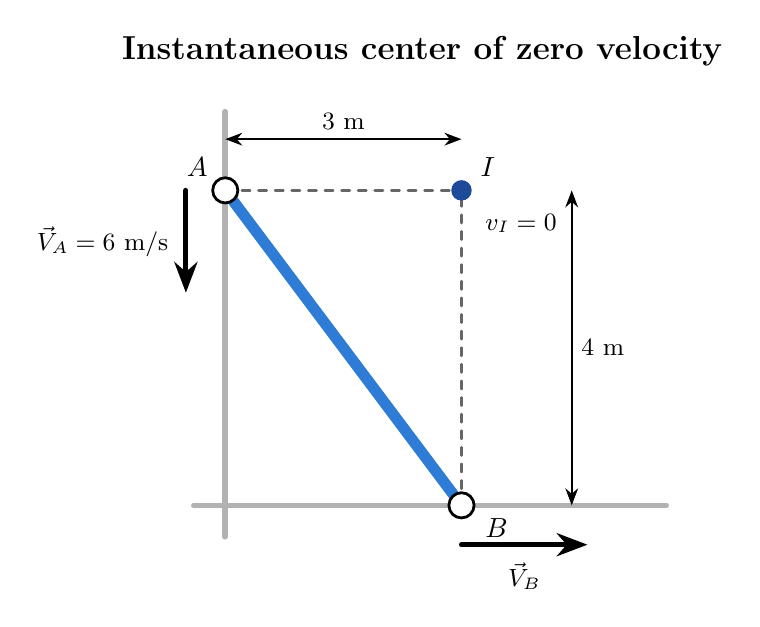
\begin{tikzpicture}[
  >=Stealth,
  line cap=round,
  every node/.style={font=\small}
]
  \coordinate (A) at (0,4);
  \coordinate (B) at (3,0);
  \coordinate (I) at (3,4);

  % Wall and floor
  \draw[gray!60, line width=2.0pt] (-0.4,0) -- (5.6,0);
  \draw[gray!60, line width=2.0pt] (0,-0.4) -- (0,5.0);

  % Rod
  \draw[rodBlue, line width=4pt] (A) -- (B);

  % Auxiliary perpendicular dashed lines (IA horizontal, IB vertical)
  \draw[black!60, dashed, line width=0.9pt] (A) -- (I);
  \draw[black!60, dashed, line width=0.9pt] (B) -- (I);

  % 3 m dimension (above AI line, in clear space)
  \draw[<->, line width=0.7pt] ($(A)+(0,0.65)$) -- ($(I)+(0,0.65)$);
  \node[above] at ($(A)!0.5!(I)+(0,0.65)$) {$3$ m};

  % 4 m dimension (right of IB line, in clear space, offset 1.4 to clear v_I=0 label)
  \draw[<->, line width=0.7pt] ($(I)+(1.4,0)$) -- ($(B)+(1.4,0)$);
  \node[right] at ($(I)!0.5!(B)+(1.4,0)$) {$4$ m};

  % V_A arrow (down, drawn outside wall to the left)
  \draw[->, line width=1.8pt, black] (-0.5,4) -- (-0.5,2.7);
  \node[anchor=east] at (-0.6,3.35) {$\vec V_A = 6\ \mathrm{m/s}$};

  % V_B arrow (right, drawn below floor)
  \draw[->, line width=1.8pt, black] (3,-0.5) -- (4.6,-0.5);
  \node[anchor=north] at (3.8,-0.6) {$\vec V_B$};

  % Slider markers at A and B (white-filled circles to mask rod end)
  \fill[white] (A) circle (0.16);
  \draw[black, line width=1pt] (A) circle (0.16);
  \fill[white] (B) circle (0.16);
  \draw[black, line width=1pt] (B) circle (0.16);

  % I marker (filled dot)
  \fill[KetteringBlue] (I) circle (0.13);

  % Point labels (placed away from arrows and lines)
  \node[font=\bfseries, anchor=south east] at ($(A)+(-0.1,0.05)$) {$A$};
  \node[font=\bfseries, anchor=north west] at ($(B)+(0.18,-0.05)$) {$B$};
  \node[font=\bfseries, anchor=south west] at ($(I)+(0.12,0.05)$) {$I$};
  \node[anchor=west] at ($(I)+(0.18,-0.42)$) {$v_I = 0$};

  % Title
  \node[font=\bfseries\large, anchor=south] at (2.5,5.45) {Instantaneous center of zero velocity};
\end{tikzpicture}
\end{document}
